% !TEX root = cha-soa.tex
\documentclass[../../main.tex]{subfiles}

\begin{document}

\section{3D and VR Visualizations}

Three-dimensional and immersive visualizations provide alternative ways to represent software structure and explore relationships between software entities. Existing approaches differ in how they organize entities in space and depict their relationships, using techniques such as hierarchical layouts, edge bundling, and semantic clustering. These approaches illustrate different ways to organize software entities and represent their relationships in three-dimensional environments.

In 2007, Wettel and Lanza~\citebibliography{Wett2007a} introduced \tool{CodeCity}, a 3D software visualization tool. Three-dimensional software visualizations can make navigation difficult, as moving freely through a 3D space can lead to disorientation. \tool{CodeCity} addresses this problem by representing a software system as a city, providing a more familiar context. Classes are represented as buildings, whose visual properties reflect software metrics. In particular, building height represents the Number of Methods (NOM), while the base size represents the Number of Attributes (NOA). Classes are grouped into districts representing packages, which can be nested to reflect the package structure. Nested packages are represented as platforms at different heights, making the package topology visible. The buildings are arranged using a modified treemap algorithm based on rectangle packing. An example is shown in \figref{fig:codeCity}.

\begin{figure}[ht]
    \centering
    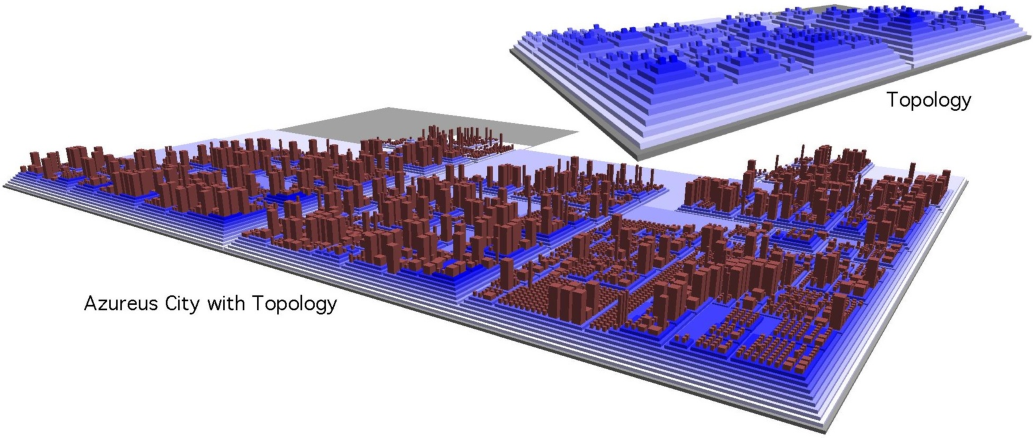
\includegraphics[width=0.84\linewidth]{figures/soa/codeCity}
    \caption[The city of Azureus and its package topology.]{The city of Azureus and its package topology~\citebibliography{Wett2007a}.}
    \label{fig:codeCity}
\end{figure}

Caserta~\etal~\citebibliography{Case2011a} extended the city metaphor to show relationships between software classes. They used the Hierarchical Edge Bundling technique proposed by Holten~\citebibliography{Holt2006a} (already presented in \secref{sec:graph-based_visualization}) and adapted it to 3D, creating \emph{3D-HEB} (\textit{3D Hierarchical Edge Bundles}). The technique bundles the edges between buildings in a software city, reducing the visual clutter that would result from drawing direct edges between individual buildings. As in the original technique, the parameter $\beta$ controls the strength of the bundling. The authors also use color to encode the direction and magnitude of the relationships. To evaluate the technique in different settings, they applied it to two types of software city layouts: nested and street layouts. This shows that 3D edge bundling can be used with different spatial organizations of the software city. An example is provided in \figref{fig:edge_bundling_3D_city}.

\begin{figure}[h]  
    \centering 
    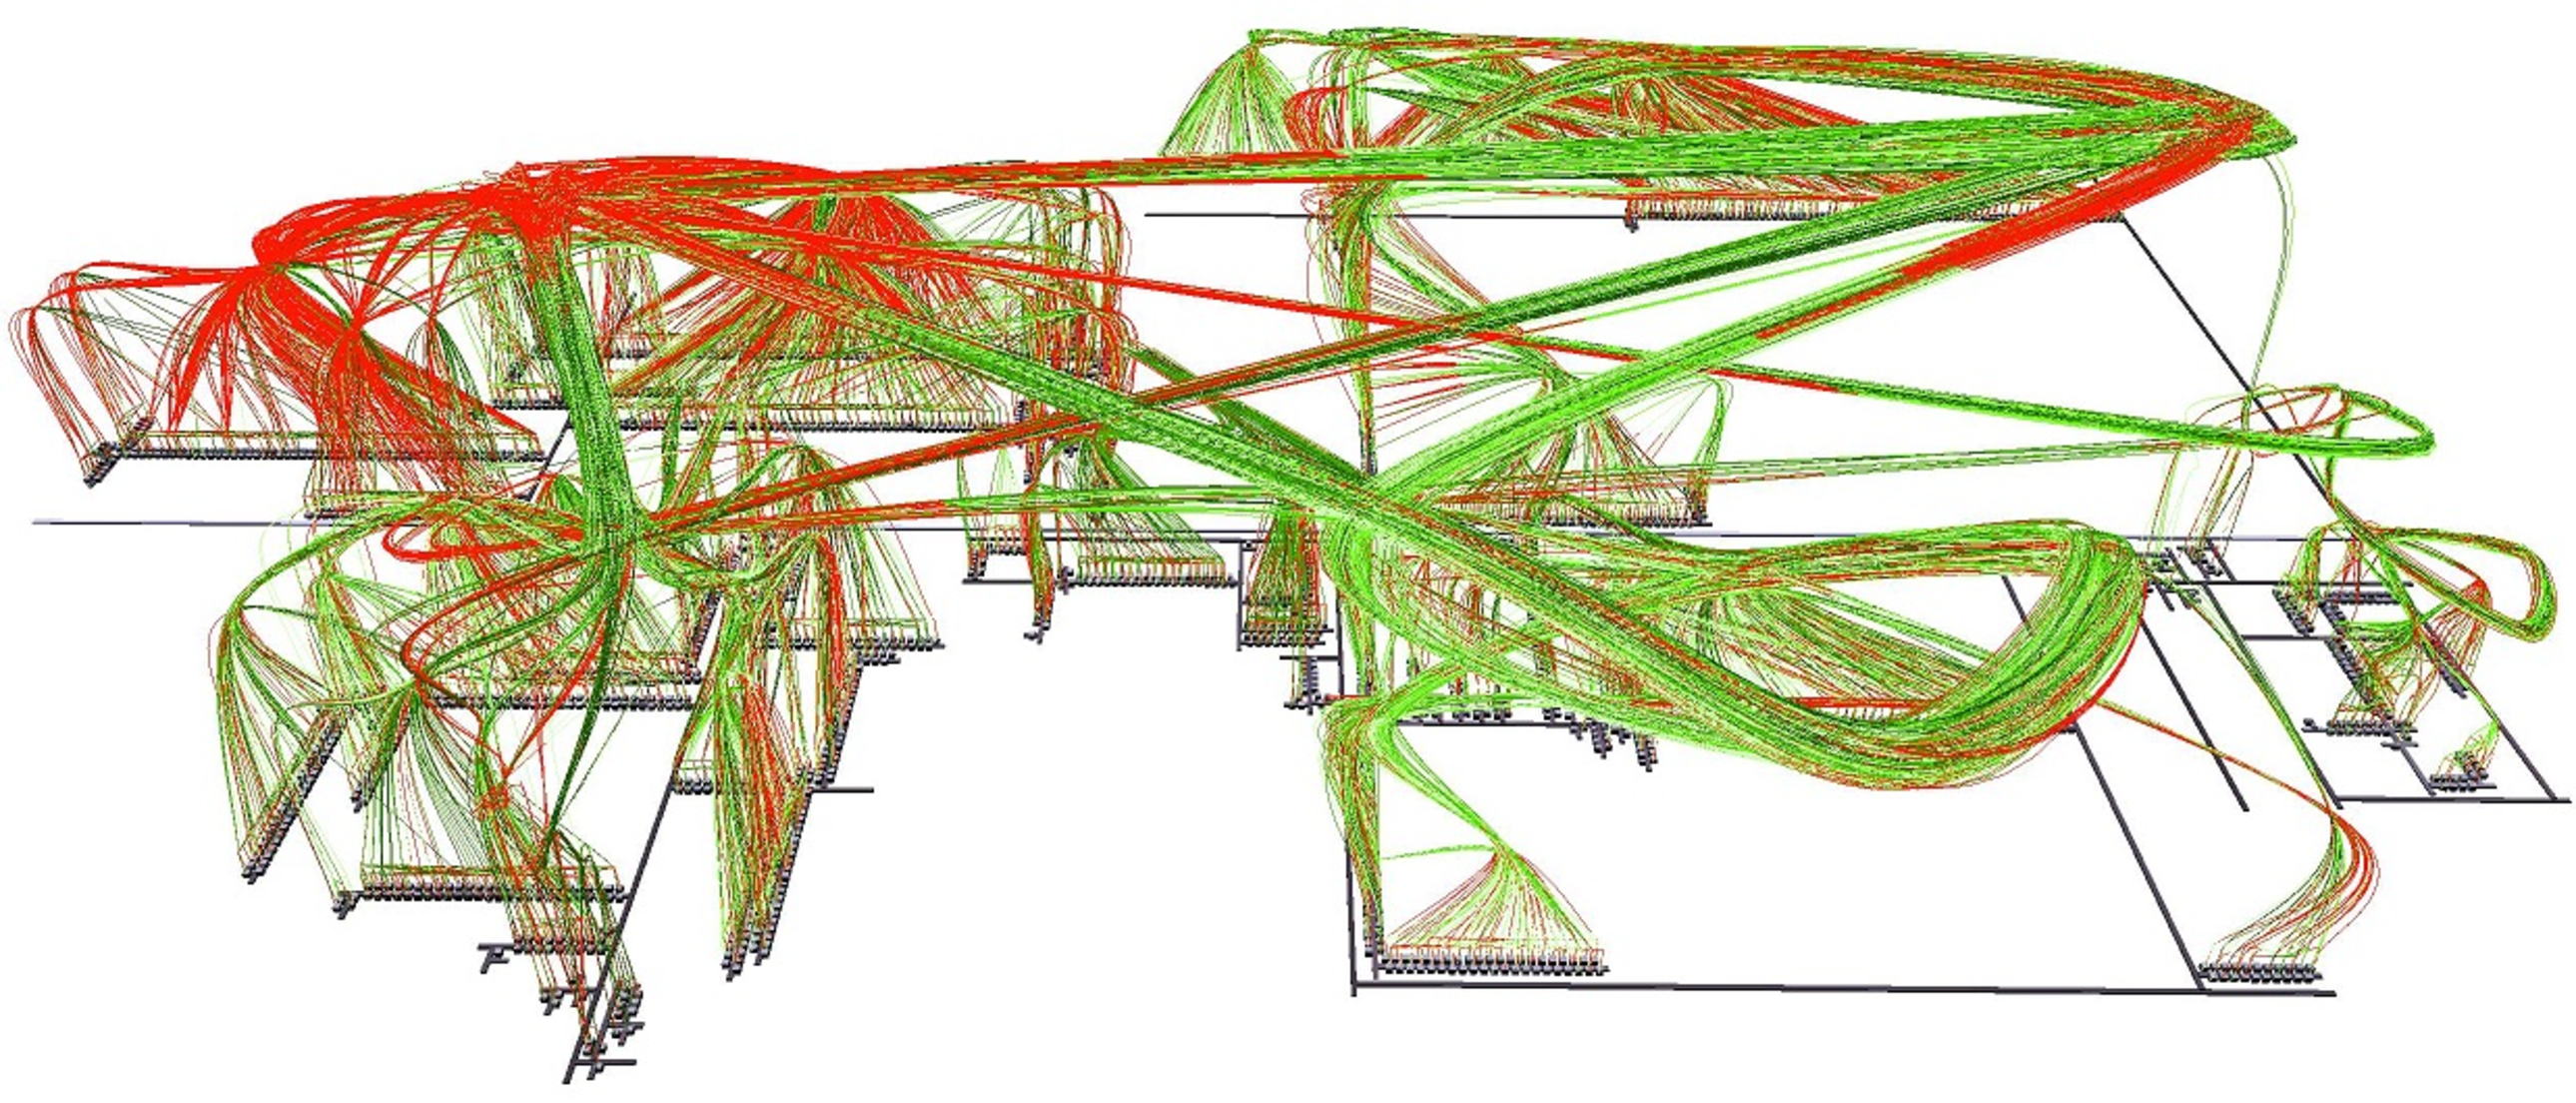
\includegraphics[width=0.84\linewidth]{figures/soa/edge_bundling_3D_city} 
    \caption[Relationships in a street-layout city.]{Relationships in a street-layout city~\citebibliography{Case2011a}.}
    \label{fig:edge_bundling_3D_city}
\end{figure}

More recently, Moreno-Lumbreras~\etal~\citebibliography{More2023a} developed a web version of \tool{CodeCity}, called \tool{BabiaXR-CodeCity}, which supports both traditional screens and Virtual Reality (VR). Unlike the original \tool{CodeCity}, the new implementation uses a spiral layout instead of a treemap. This choice makes it easier to represent software evolution, since new elements can be added without moving the existing ones. The authors compared the two visualization modes through two experiments, involving 24 and 26 participants from academia and industry. The participants were asked to perform some tasks using the same visualization either on-screen or in VR. The results showed that VR participants completed the tasks significantly faster, sometimes in about half the time required by on-screen participants. At the same time, their correctness was comparable to that of on-screen participants, and in the second experiment it was even higher for several tasks. The authors suggest that the faster results in VR may be related to its more natural spatial interaction, such as moving the head or body to inspect the visualization, compared with navigating a 3D scene using a keyboard and mouse.

Unlike \tool{CodeCity} and \tool{BabiaXR-CodeCity}, which mainly use physical structures such as packages to organize software entities, Hoff~\etal~\citebibliography{Hoff2024a} proposed \tool{ISA} (\textit{Immersive Software Archaeology}), a VR tool that organizes software according to its logical architecture. ISA first uses automated clustering to identify groups of classes that form cohesive architectural components. These components are represented at different levels of abstraction, which users can navigate from the architectural level down to the design level and back using semantic zoom. At the highest level, architectural components are represented as planets in a solar system. As users zoom in, these components are divided into continents and cities, with buildings representing classes. At the class level, the floors of each building encode method metrics, such as cognitive complexity. An example of the \tool{ISA} interface is shown in \figref{fig:softwareArcheology}. ISA also provides interactive 3D relationship graphs that allow users to explore dependencies between software entities. A controlled experiment with 54 participants showed that grouping classes according to logical architectural components, rather than only their physical structure, improved information retrieval and helped participants build better mental models of unfamiliar software systems.

\begin{figure}[h]
    \centering
    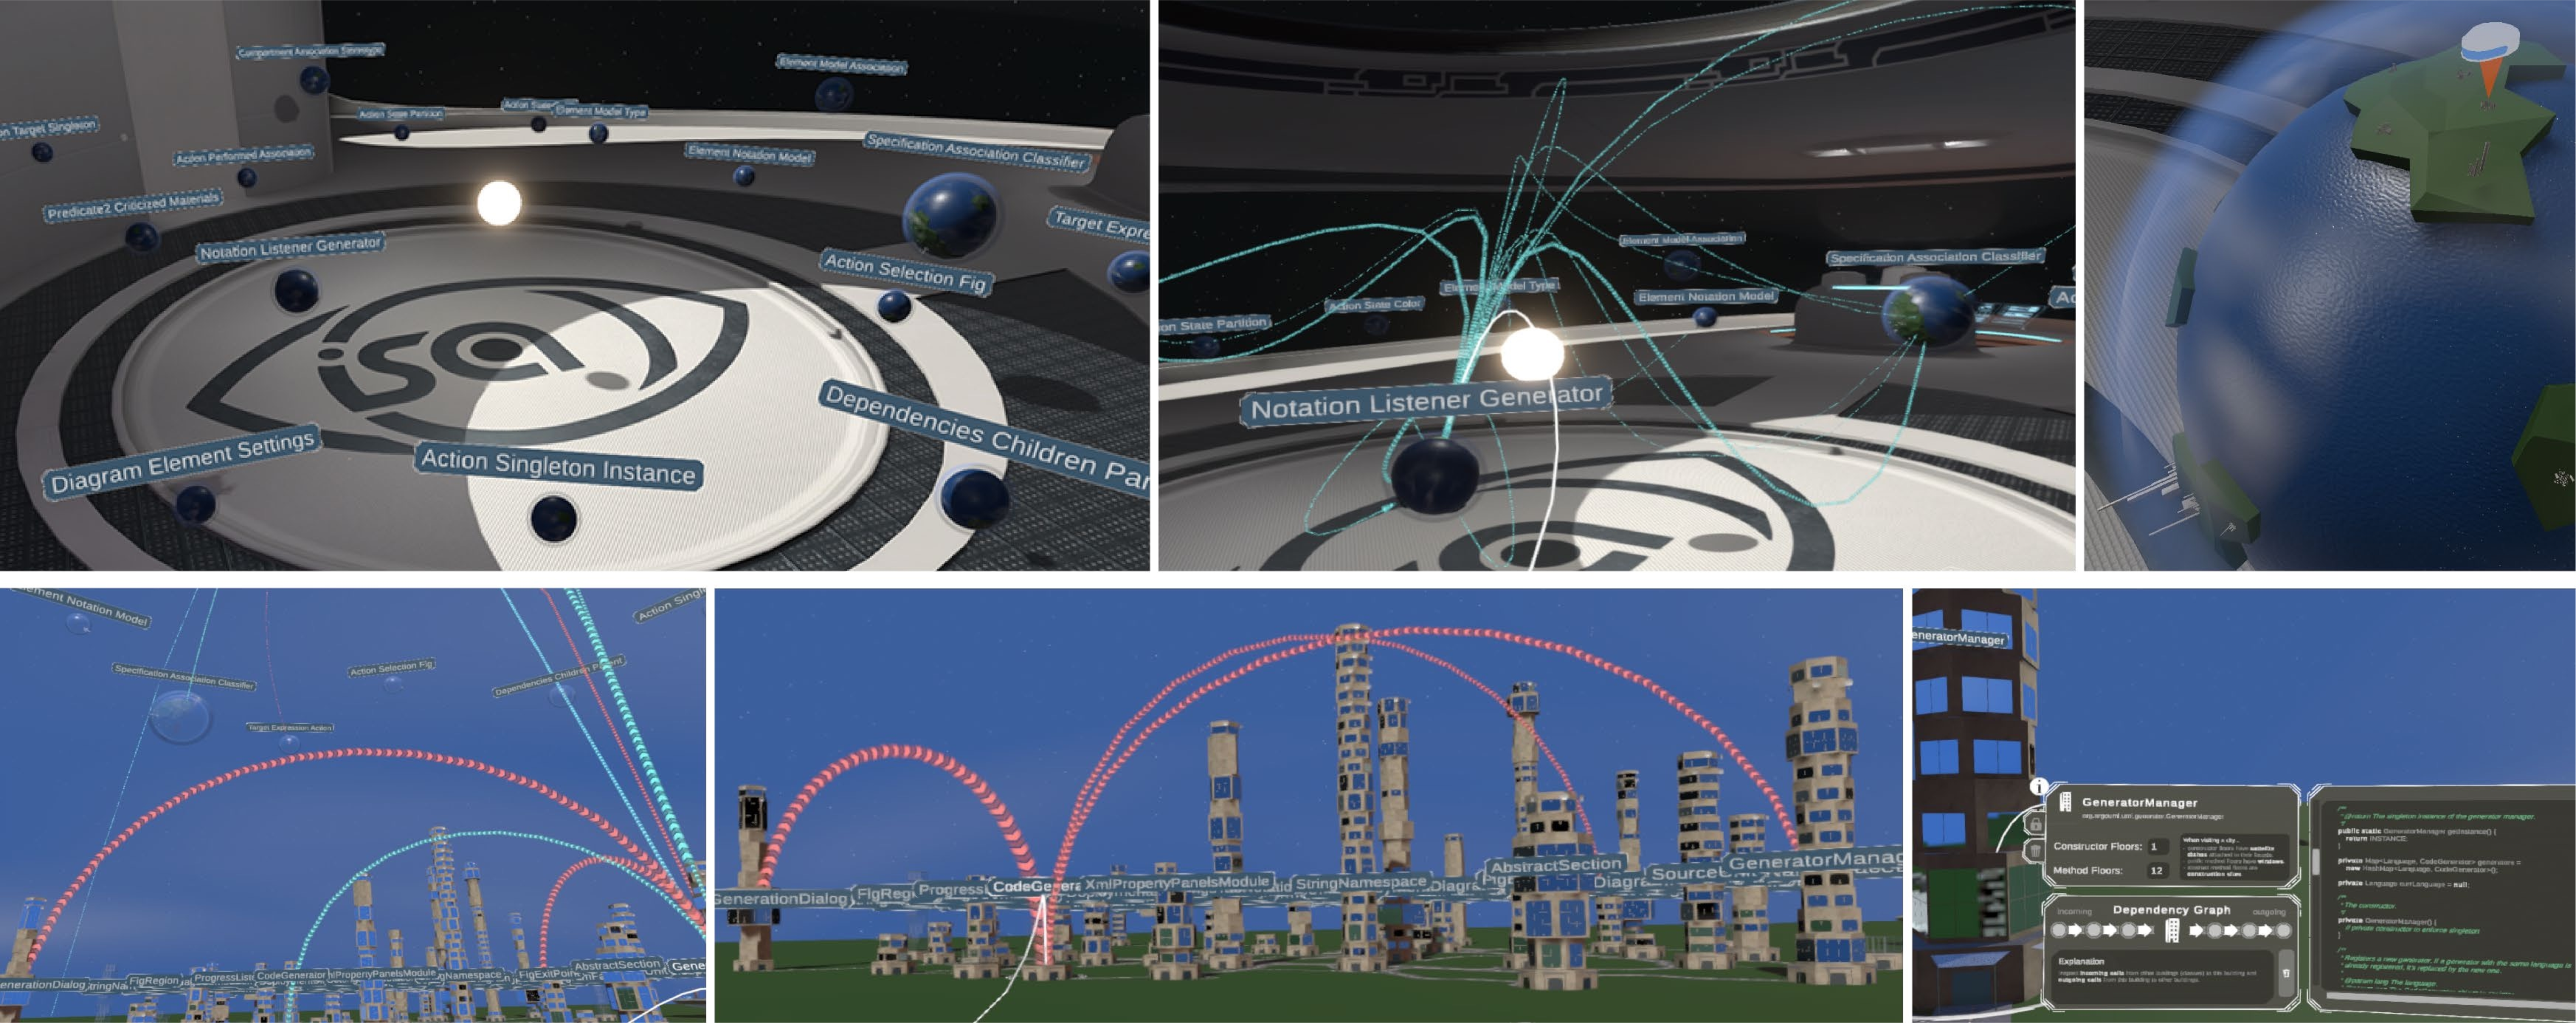
\includegraphics[width=0.8\linewidth]{figures/soa/softwareArcheology}
    \caption[\tool{ISA}'s VR application.]{\tool{ISA}'s VR application~\citebibliography{Hoff2024a}.}
    \label{fig:softwareArcheology}
\end{figure}

While VR can make software visualization easier to explore, configuring the visualization itself can still be difficult. Traditional tools often use external 2D interfaces or Domain-Specific Languages (DSLs), forcing users to leave the VR environment or interact with 2D menus inside the virtual space. To address this problem, Giannaccari~\etal~\citebibliography{Gian2024a} introduced \tool{IVaR-NI}, a tool that allows users to customize visualizations directly in VR. Instead of using traditional menus, \tool{IVaR-NI} represents meta-entities in the system as 3D shapes. Users can interact with these objects using VR controllers to configure properties such as layout, size, and color, to define the desired visualization. The tool also provides an interactive preview of the visualization, allowing users to immediately see the effect of their changes.

\end{document}